\ylDisplay{Fookuskaugus} % Ülesande nimi
{Eero Vaher} % Autor
{piirkonnavoor} % Voor
{2015} % Aasta
{G 8} % Ülesande nr.
{6} % Raskustase
{
% Teema: Geomeetriline-optika
\ifStatement
Õhukese tasanõgusa läätse parem külg on hõbetatud. Kui suur on sellise optilise elemendi fookuskaugus $f$ vasakult langeva valguse jaoks? Läätse nõgusa osa kõverusraadius on $R$, läätse materjali murdumisnäitaja ümbritseva keskkonna suhtes on $n$.

\begin{center}
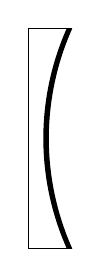
\begin{tikzpicture}[scale=0.7, transform shape]
\def\tmp{65.92}
\fill [black] (0.7,2) arc[start angle=90+\tmp, end angle=270-\tmp,radius=4.9] -- (0.8,-2) -- (0.8,-2) arc[start angle=270-\tmp, end angle=90+\tmp,radius=4.9] -- (0.7,2);
\draw (0.8,-2) -- (0,-2) -- (0,2) -- (0.8,2);
\end{tikzpicture}
\end{center}
\fi


\ifHint
Läätse fookuskauguse leidmiseks tasub vaadelda valguskimpu, mille suund on paralleelne optilise peateljega. Sellisel juhul tekitavad kiired näilise kujutise läätse fookusesse.
\fi


\ifSolution
Langegu läätsele vasakult valguskiir, mille suund on paralleelne optilise teljega ning mille kaugus sellest on $d$. Läätse sisenedes valgus oma levimissuunda ei muuda, kuna langeb läätsele selle pinnaga risti. Hõbetatud pind toimib kumerpeeglina, mille fookuskaugus on $\frac{R}{2}$. Kui peegeldunud valguskiire nurk optilise peatelje suhtes on $\alpha$, siis läätsest väljunud kiire ning optilise peatelje vaheline nurk on murdumisseaduse põhjal $\sin\gamma=n\sin\alpha$. Kuna lääts on õhuke, asetsevad punktid, kus valguskiir peegeldus ning kus see murdus, üksteisele väga lähedal. Seetõttu võime kirjutada
\[ d=\frac{R}{2}\tan\alpha=f\tan\gamma. \]
Õhukese läätse korral on selle nõgusa osa kõverusraadius oluliselt suurem fookuskaugusest, mis lubab kasutada väikeste nurkade lähendust ehk $\alpha\approx\sin\alpha\approx\tan\alpha$ ning $\gamma\approx\sin\gamma\approx\tan\gamma$. Tulemuseks saame
\[ f=\frac{R}{2n}. \]
Tasub teada, et avaldis sfäärilise peegli fookuskauguse jaoks kehtibki ainult väikeste peegeldumisnurkade korral. Suurte peegeldumisnurkade korral ilmneb sfääriline aberratsioon ning ei ole võimalik rääkida ühest fookusest.

\begin{center}
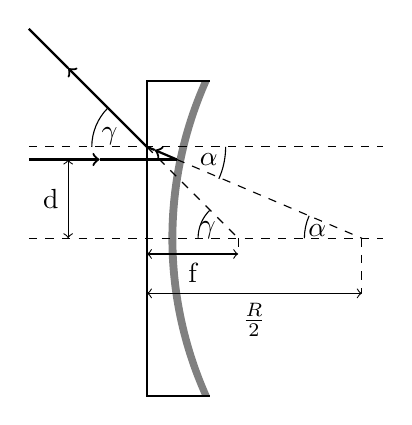
\begin{tikzpicture}[scale=1]
\def\tmp{65.92}
\fill [gray] (0.7,2) arc (90+\tmp:270-\tmp:4.9) -- (0.8,-2) -- (0.8,-2) arc (270-\tmp:90+\tmp:4.9) -- (0.7,2);
\draw[thick] (0.8,-2) -- (0,-2) -- (0,2) -- (0.8,2);
\draw[dashed] (-1.5,0) -- (3,0);
\draw[->,thick] (-1.5,1) -- (-0.6,1);
\draw[thick] (-0.6,1) -- (0.38,1);
\draw[dashed] (0.38,1) -- (2.73,0);
\draw[->,thick] (0.38,1) -- (0.1,1.12);
\draw[thick] (0.1,1.12) -- (0,1.16);
\draw[->,thick] (0,1.16) -- (-1,2.16);
\draw[thick] (-1,2.16) -- (-1.5,2.66);
\draw[dashed] (0,1.16) -- (1.16,0);
\draw[<->] (-1,0) -- (-1,1);
\node [left] at (-1,0.5) {d};
\draw[dashed] (-1.5,1.16) -- (3,1.16);
\node [left] at (-0.25,1.3) {$\gamma$};
\draw (-0.7,1.16) arc (180:135:0.7);
\node [right] at (0.55,1) {$\alpha$};
\draw (1,1.16) arc (0:-24:1);
\draw[dashed] (1.16,0) -- (1.16,-0.2);
\draw[<->] (0,-0.2) -- (1.16,-0.2);
\node [below] at (0.58,-0.2) {f}; 
\draw[dashed] (2.73,0) -- (2.73,-0.7);
\draw[<->] (0,-0.7) -- (2.73,-0.7);
\node[below] at (1.36,-0.7) {$\frac{\text{R}}{2}$};
\node[left] at (2.4,0.1) {$\alpha$};
\draw (2,0) arc (180:156:0.7);
\node[left] at (1,0.1) {$\gamma$};
\draw (0.65,0) arc (180:135:0.5);
\end{tikzpicture}
\end{center}
\fi


\ifEngStatement
% Problem name: Focal length
The left face of a thin lens is flat while the right face is concave and silvered. How big is the focal length $f$ of such an optical element for a light falling from the left? The radius of the lens’s concave part is $R$, the refractive index of the lens with respect to the surrounding environment is $n$.
\begin{center}
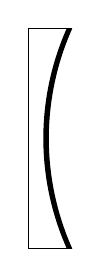
\begin{tikzpicture}[scale=0.7, transform shape]
\def\tmp{65.92}
\fill [black] (0.7,2) arc[start angle=90+\tmp, end angle=270-\tmp,radius=4.9] -- (0.8,-2) -- (0.8,-2) arc[start angle=270-\tmp, end angle=90+\tmp,radius=4.9] -- (0.7,2);
\draw (0.8,-2) -- (0,-2) -- (0,2) -- (0.8,2);
\end{tikzpicture}
\end{center}
\fi


\ifEngHint
To find the focal point of the lens you should observe a beam of light that has the direction parallel to the optical main axis. In this case the rays make a virtual image at the focal point of the lens.
\fi


\ifEngSolution
Let us propose a light ray that is coming from the left falls on the lens, it has the direction parallel to the optical axis and is at a distance $d$ from it. Entering the lens the light does not change its travel direction because it falls on the lens perpendicularly to its surface. The silvered surface acts as a convex mirror that has a focal length $\frac{R}{2}$. If the reflected ray is at an angle $\alpha$ with respect to the optical axis then the angle between the ray exiting the lens and the optical axis according to the law of refraction is $\sin\gamma=n\sin\alpha$. Because the lens is thin then the points where the light ray reflected and where it refracted are positioned very close to each other. Therefore we can write
\[ d=\frac{R}{2}\tan\alpha=f\tan\gamma. \] 
In the case of a thin lens the radius of its concave part is significantly bigger from the focal length, this allows us to use the paraxial approximation $\alpha\approx\sin\alpha\approx\tan\alpha$ and $\gamma\approx\sin\gamma\approx\tan\gamma$. In result we get
\[ f=\frac{R}{2n}. \] 
It should be known that the expression for the focal length of a spherical mirror only applies for small angles of reflection. In the case of big angles of reflection a spherical aberration occurs and it is not possible to talk about one focal point. 
\begin{center}
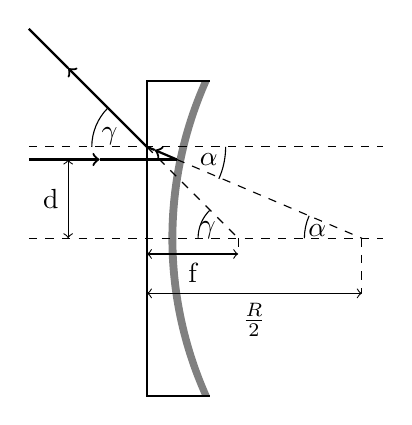
\begin{tikzpicture}[scale=1]
\def\tmp{65.92}
\fill [gray] (0.7,2) arc (90+\tmp:270-\tmp:4.9) -- (0.8,-2) -- (0.8,-2) arc (270-\tmp:90+\tmp:4.9) -- (0.7,2);
\draw[thick] (0.8,-2) -- (0,-2) -- (0,2) -- (0.8,2);
\draw[dashed] (-1.5,0) -- (3,0);
\draw[->,thick] (-1.5,1) -- (-0.6,1);
\draw[thick] (-0.6,1) -- (0.38,1);
\draw[dashed] (0.38,1) -- (2.73,0);
\draw[->,thick] (0.38,1) -- (0.1,1.12);
\draw[thick] (0.1,1.12) -- (0,1.16);
\draw[->,thick] (0,1.16) -- (-1,2.16);
\draw[thick] (-1,2.16) -- (-1.5,2.66);
\draw[dashed] (0,1.16) -- (1.16,0);
\draw[<->] (-1,0) -- (-1,1);
\node [left] at (-1,0.5) {d};
\draw[dashed] (-1.5,1.16) -- (3,1.16);
\node [left] at (-0.25,1.3) {$\gamma$};
\draw (-0.7,1.16) arc (180:135:0.7);
\node [right] at (0.55,1) {$\alpha$};
\draw (1,1.16) arc (0:-24:1);
\draw[dashed] (1.16,0) -- (1.16,-0.2);
\draw[<->] (0,-0.2) -- (1.16,-0.2);
\node [below] at (0.58,-0.2) {f}; 
\draw[dashed]  (2.73,0) -- (2.73,-0.7);
\draw[<->] (0,-0.7) -- (2.73,-0.7);
\node[below] at (1.36,-0.7) {$\frac{\text{R}}{2}$};
\node[left] at (2.4,0.1) {$\alpha$};
\draw (2,0) arc (180:156:0.7);
\node[left] at (1,0.1) {$\gamma$};
\draw (0.65,0) arc (180:135:0.5);
\end{tikzpicture}
\end{center}
\fi
}